\XtoCBlock{Sum}
\label{block:Sum}
\begin{figure}[H]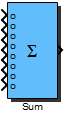
\includegraphics{Sum}\end{figure} 

\begin{XtoCtabular}{Inports}
In1 & Input \#1\tabularnewline
\hline
In2 & Input \#2\tabularnewline
\hline
In3 & Input \#3\tabularnewline
\hline
In4 & Input \#4\tabularnewline
\hline
In5 & Input \#5\tabularnewline
\hline
In6 & Input \#6\tabularnewline
\hline
In7 & Input \#7\tabularnewline
\hline
In8 & Input \#8\tabularnewline
\hline
\end{XtoCtabular}


\begin{XtoCtabular}{Outports}
Out & Result\tabularnewline
\hline
\end{XtoCtabular}

\begin{XtoCMaskParamTabular}{Mask Parameters}
\rowcolor[gray]{0.8}\textbf{Name} & \textbf{ID} & \textbf{Description}\tabularnewline\hline
In1 & 1 & Input \#1\tabularnewline
\hline
In2 & 2 & Input \#2\tabularnewline
\hline
In3 & 3 & Input \#3\tabularnewline
\hline
In4 & 4 & Input \#4\tabularnewline
\hline
In5 & 5 & Input \#5\tabularnewline
\hline
In6 & 6 & Input \#6\tabularnewline
\hline
In7 & 7 & Input \#7\tabularnewline
\hline
In8 & 8 & Input \#8\tabularnewline
\hline
\end{XtoCMaskParamTabular}

\subsubsection*{Description:}
Sum of inputs:

    + ... Input will be added to result.

    - ... Input will be subtracted from result.

    0 ... Input will be ignored.

\subsubsection*{Implementations:}
\begin{tabular}{l l}
\textbf{FiP8} & 8 Bit Fixed Point Implementation\tabularnewline
\textbf{FiP16} & 16 Bit Fixed Point Implementation\tabularnewline
\textbf{FiP32} & 32 Bit Fixed Point Implementation\tabularnewline
\textbf{Float32} & 32 Bit Floating Point Implementation\tabularnewline
\textbf{Float64} & 64 Bit Floating Point Implementation\tabularnewline
\end{tabular}

\XtoCImplementation{FiP8}
\nopagebreak[0]

8 Bit Fixed Point Implementation

\begin{XtoCtabular}{Inports Data Type}
In1 & int8\tabularnewline
\hline
In2 & int8\tabularnewline
\hline
In3 & int8\tabularnewline
\hline
In4 & int8\tabularnewline
\hline
In5 & int8\tabularnewline
\hline
In6 & int8\tabularnewline
\hline
In7 & int8\tabularnewline
\hline
In8 & int8\tabularnewline
\hline
\end{XtoCtabular}

\begin{XtoCtabular}{Outports Data Type}
Out & int8\tabularnewline
\hline
\end{XtoCtabular}

\ifdefined \AddTestReports
\InputIfFileExists{\XcHomePath/Library/Math/Doc/Test-Results/Test_Sum_FiP8.tex}{}{}
\fi
\XtoCImplementation{FiP16}
\nopagebreak[0]

16 Bit Fixed Point Implementation

\begin{XtoCtabular}{Inports Data Type}
In1 & int16\tabularnewline
\hline
In2 & int16\tabularnewline
\hline
In3 & int16\tabularnewline
\hline
In4 & int16\tabularnewline
\hline
In5 & int16\tabularnewline
\hline
In6 & int16\tabularnewline
\hline
In7 & int16\tabularnewline
\hline
In8 & int16\tabularnewline
\hline
\end{XtoCtabular}

\begin{XtoCtabular}{Outports Data Type}
Out & int16\tabularnewline
\hline
\end{XtoCtabular}

\ifdefined \AddTestReports
\InputIfFileExists{\XcHomePath/Library/Math/Doc/Test-Results/Test_Sum_FiP16.tex}{}{}
\fi
\XtoCImplementation{FiP32}
\nopagebreak[0]

32 Bit Fixed Point Implementation

\begin{XtoCtabular}{Inports Data Type}
In1 & int32\tabularnewline
\hline
In2 & int32\tabularnewline
\hline
In3 & int32\tabularnewline
\hline
In4 & int32\tabularnewline
\hline
In5 & int32\tabularnewline
\hline
In6 & int32\tabularnewline
\hline
In7 & int32\tabularnewline
\hline
In8 & int32\tabularnewline
\hline
\end{XtoCtabular}

\begin{XtoCtabular}{Outports Data Type}
Out & int32\tabularnewline
\hline
\end{XtoCtabular}

\ifdefined \AddTestReports
\InputIfFileExists{\XcHomePath/Library/Math/Doc/Test-Results/Test_Sum_FiP32.tex}{}{}
\fi
\XtoCImplementation{Float32}
\nopagebreak[0]

32 Bit Floating Point Implementation

\begin{XtoCtabular}{Inports Data Type}
In1 & float32\tabularnewline
\hline
In2 & float32\tabularnewline
\hline
In3 & float32\tabularnewline
\hline
In4 & float32\tabularnewline
\hline
In5 & float32\tabularnewline
\hline
In6 & float32\tabularnewline
\hline
In7 & float32\tabularnewline
\hline
In8 & float32\tabularnewline
\hline
\end{XtoCtabular}

\begin{XtoCtabular}{Outports Data Type}
Out & float32\tabularnewline
\hline
\end{XtoCtabular}

\ifdefined \AddTestReports
\InputIfFileExists{\XcHomePath/Library/Math/Doc/Test-Results/Test_Sum_Float32.tex}{}{}
\fi
\XtoCImplementation{Float64}
\nopagebreak[0]

64 Bit Floating Point Implementation

\begin{XtoCtabular}{Inports Data Type}
In1 & float64\tabularnewline
\hline
In2 & float64\tabularnewline
\hline
In3 & float64\tabularnewline
\hline
In4 & float64\tabularnewline
\hline
In5 & float64\tabularnewline
\hline
In6 & float64\tabularnewline
\hline
In7 & float64\tabularnewline
\hline
In8 & float64\tabularnewline
\hline
\end{XtoCtabular}

\begin{XtoCtabular}{Outports Data Type}
Out & float64\tabularnewline
\hline
\end{XtoCtabular}

\ifdefined \AddTestReports
\InputIfFileExists{\XcHomePath/Library/Math/Doc/Test-Results/Test_Sum_Float64.tex}{}{}
\fi
